\part{Conception d'ensemble}
\setcounter{section}{0}

\section{Modèles conceptuels de données} 

\subsection{Données clients et produits} 

\begin{figure}[H]
\centering
\includegraphics[width=\textwidth]{figures/mcd/MCD_Clients_Produits}
\caption{MCD Clients Produits}
\end{figure}

On a distingué quatre proximités au niveau de la sémantique des données, le client, la personne, le produit et la structure. \\

Tout ce qui est du domaine de l'humain est dans l'objet métier \textbf{Personne}, soit l'individu ainsi que son ou ses lieux d'habitation. À ne pas mélanger avec les différents individus qui ont un rôle, comme l'agent et le client. Le cycle de vie d'une personne est bien différent de celui du rôle qu'elle joue. \\

Ce qui est du domaine des produits et des services sont regroupés dans l'objet métier \textbf{Produit}. On y trouve l'entité produit avec ses offres associées et la segmentation des individus qui est primordiale pour une offre (proximité fonctionnelle). \\

Toute la structuration de la société, soit les agences et les agents y travaillant ont aussi été rapprochés afin de former l'objet métier \textbf{Structure}. Même si le cycle de vie peut différer, on a une proximité fonctionnelle. Ainsi pour limiter les interactions entre blocs nous avons fait le choix de le laisser regroupé ainsi. \\

Enfin, une personne ayant le rôle de client n'existe que si cette dernière possède des comptes, donc la sémantique des données est très proche. On a alors l'objet métier \textbf{Client}. Il est plus pertinent de garder les différentes associations multiples (\textit{0,n}) entre \textbf{Client} et les autres blocs, car c'est lui qui est au centre. On aura par exemple plus de liaison dans le sens \textbf{Client} / \textbf{Produit} que l'inverse.

\subsection{Données commerciales}

\begin{figure}[H]
\centering
\includegraphics[width=\textwidth]{figures/mcd/MCD_Commercial}
\caption{MCD Commercial}
\end{figure}

\section{Diagramme d’état de l'objet métier \bf{contact}}

\begin{figure}[H]
\noindent\makebox[\textwidth]{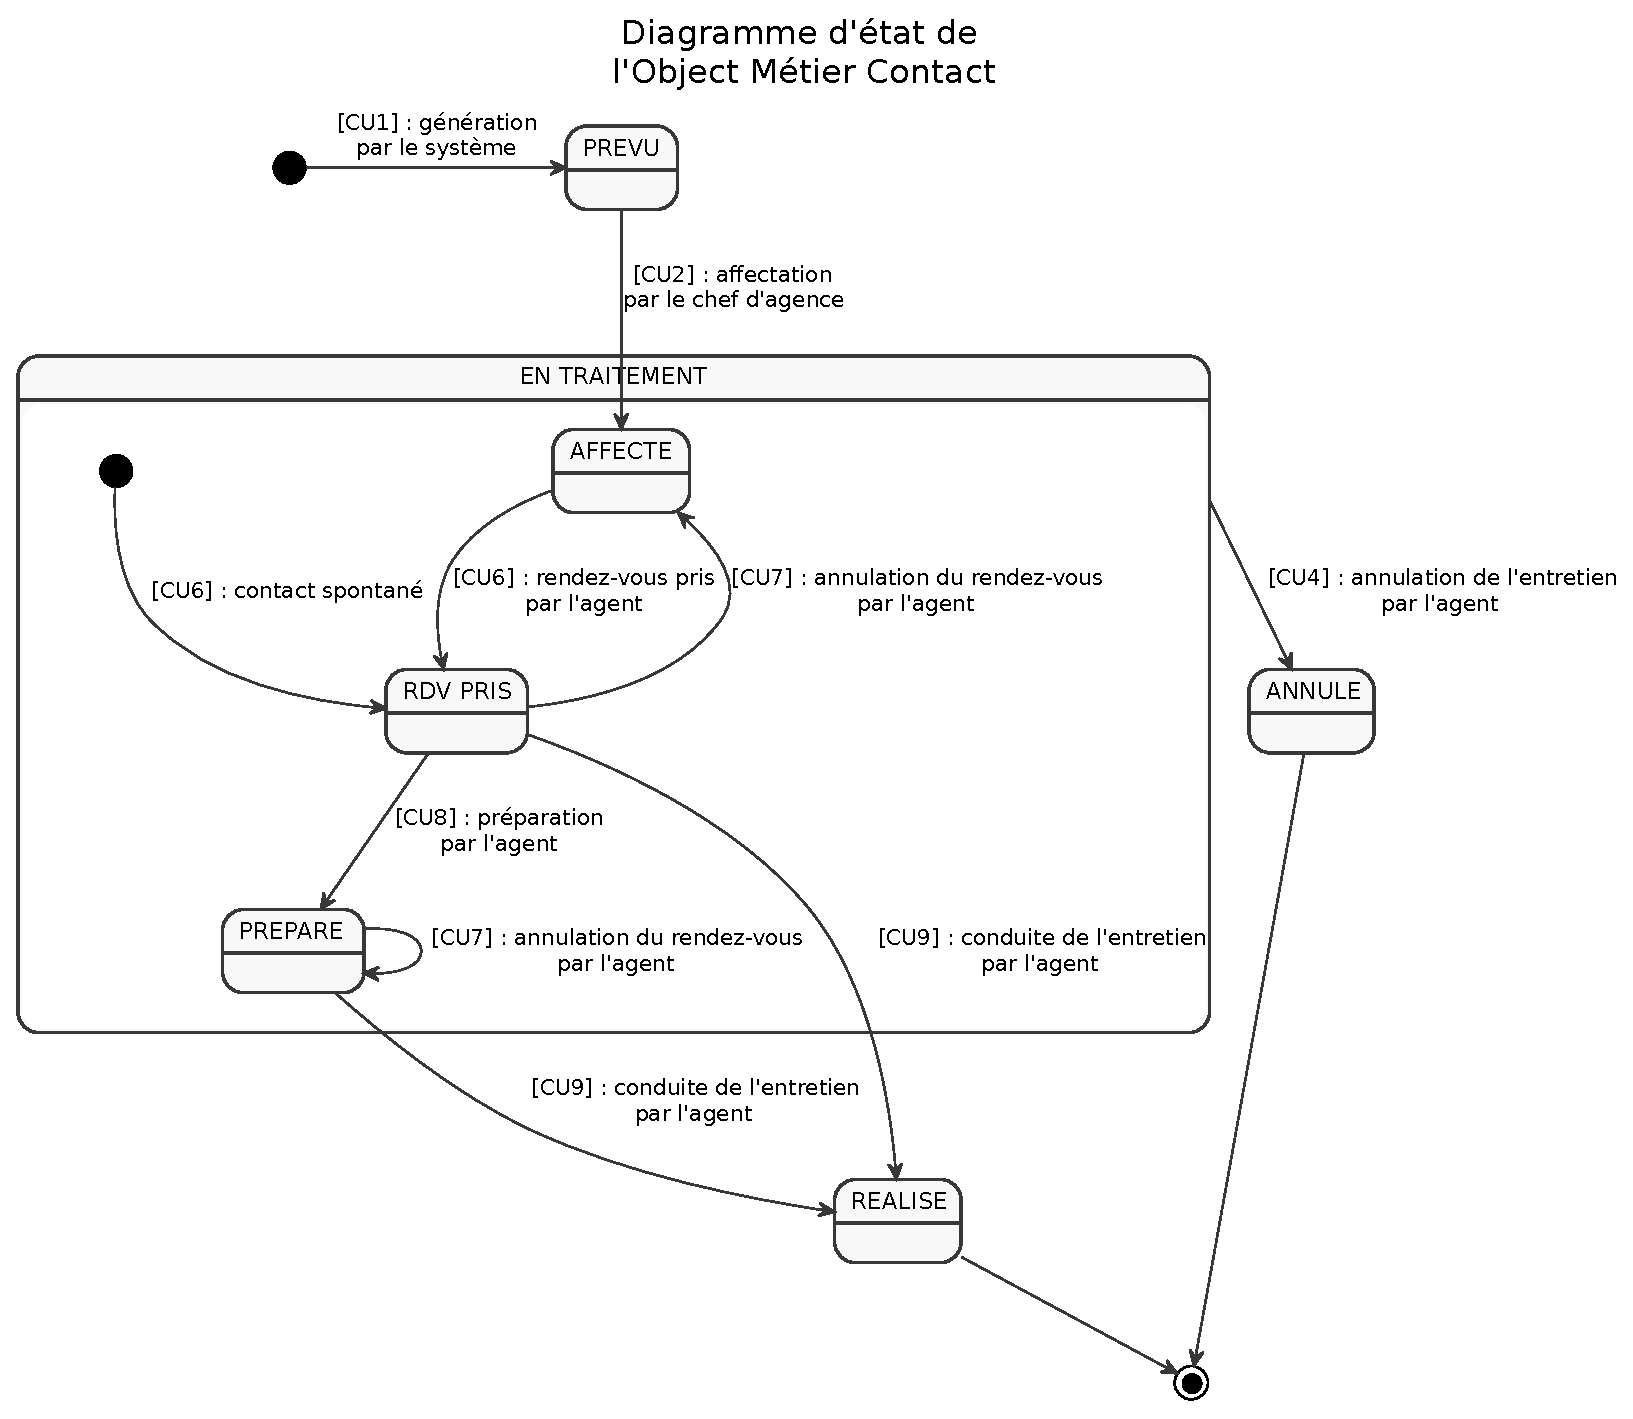
\includegraphics[width=18cm]{figures/eps/diag_etats_contact}}
\caption{Diagramme d'état de l'objet métier contact}
\end{figure}

\section{Choix  de  l’environnement  technique}
L’environnement  technique  déjà  retenu  par  la 
Maîtrise d’Ouvrage (MOA) de la banque est une architecture C/S n-tiers. 